\documentclass[11pt,a4paper]{article}

\usepackage[utf8]{inputenc}
\usepackage[T1]{fontenc}
\usepackage[brazilian]{babel}
\usepackage{geometry}
\usepackage{graphicx}
\usepackage{booktabs}
\usepackage{amsmath}
\usepackage{float}
\usepackage{hyperref}

\geometry{margin=2.4cm}
\hypersetup{hidelinks}
\setlength{\parskip}{0.45em}
\setlength{\parindent}{0pt}

\title{DBO na entrada com JEPA\\[0.3em]
\large Previsão no espaço do embedding}
\author{SoftSensor}
\date{16 de outubro de 2026}

\begin{document}
\maketitle

\section{Objetivo}

Estimar a DBO na entrada, \texttt{DBO-E}, a partir de 10 leituras de DQO (\texttt{DQO-E}) e de SST (\texttt{SS-E}). A fila é a mesma da rede recorrente: o dia estimado e as nove leituras anteriores disponíveis.

JEPA (\emph{Joint-Embedding Predictive Architecture}) treina a previsão no espaço de um vetor, não no número da DBO. Um codificador transforma a fila em um vetor. Outro transforma a DBO em um vetor do mesmo tamanho. Um preditor tenta reproduzir o vetor da DBO a partir do vetor da fila. A perda é a distância entre esses dois vetores. Uma penalidade de variância empurra cada eixo do vetor para não encolher até zero. A DBO numérica sai depois, por uma regressão linear lida no vetor da fila. Na hora do teste o codificador da DBO não é usado: a planta só oferece DQO e SST.

\section{Dados e protocolo}

O corte temporal é o da RNN, para os dois resultados se referirem aos mesmos dias. São 498 dias completos na entrada. As 389 janelas mais antigas treinam. As 100 mais recentes, de 29 de maio a 29 de outubro de 1991, testam. A validação cruzada é temporal, com 5 partições, e escolhe a configuração pelo MAE dessa reta de leitura.

A grade cobre larguras ocultas de 16 e 32, embeddings de 8 e 16, e taxas \(10^{-3}\) e \(10^{-2}\). O peso da penalidade de variância é 0,2. O ajuste final repete, em todas as janelas de treino, o número mediano de épocas da configuração vencedora. A reta de leitura é ajustada só no treino.

\section{Resultados}

A validação escolhe largura 32, embedding de 8 e taxa \(10^{-2}\). O MAE nas partições é 46,29, com desvio 6,05. A parada ocorre em 1 época. A rede tem 1816 parâmetros. As oito configurações ficam entre 46,29 e 50,60 de MAE, e todas param em no máximo 16 épocas. Alongar o treino do embedding piora a DBO na validação.

\begin{table}[H]
\centering
\caption{Erro nos mesmos 100 dias finais usados na RNN.}
\begin{tabular}{lrrr}
\toprule
Modelo & MAE & RMSE & \(R^{2}\) \\
\midrule
Média do treino & 40,88 & 48,15 & $-$0,73 \\
Linear da leitura atual & 33,13 & 40,75 & $-$0,24 \\
Linear das 10 leituras & 34,08 & 42,83 & $-$0,37 \\
RNN & 32,00 & 40,68 & $-$0,23 \\
JEPA & 32,78 & 41,39 & $-$0,28 \\
\bottomrule
\end{tabular}
\end{table}

A linha da RNN é a do relatório anterior, neste mesmo corte. Ela não foi retreinada aqui.

No teste, a previsão do JEPA vai de 122,15 a 303,87, e a DBO observada vai de 84 a 277. O resíduo médio é $-$22,06. A mediana do erro absoluto é 27,42 e o percentil 90 é 70,11. Em 55 dos 100 dias o erro absoluto fica até 30; em 76 dias, até 50.

No treino, o desvio médio do embedding da fila é 0,528. O da DBO é 0,061 e o do vetor previsto é 0,119. A penalidade pedia desvio perto de 1. A correlação média, eixo a eixo, entre o vetor previsto e o vetor da DBO é $-$0,02. O erro quadrático entre eles é 0,022, pequeno porque os dois vetores estão encolhidos, não porque um acompanha o outro.

\begin{figure}[H]
\centering
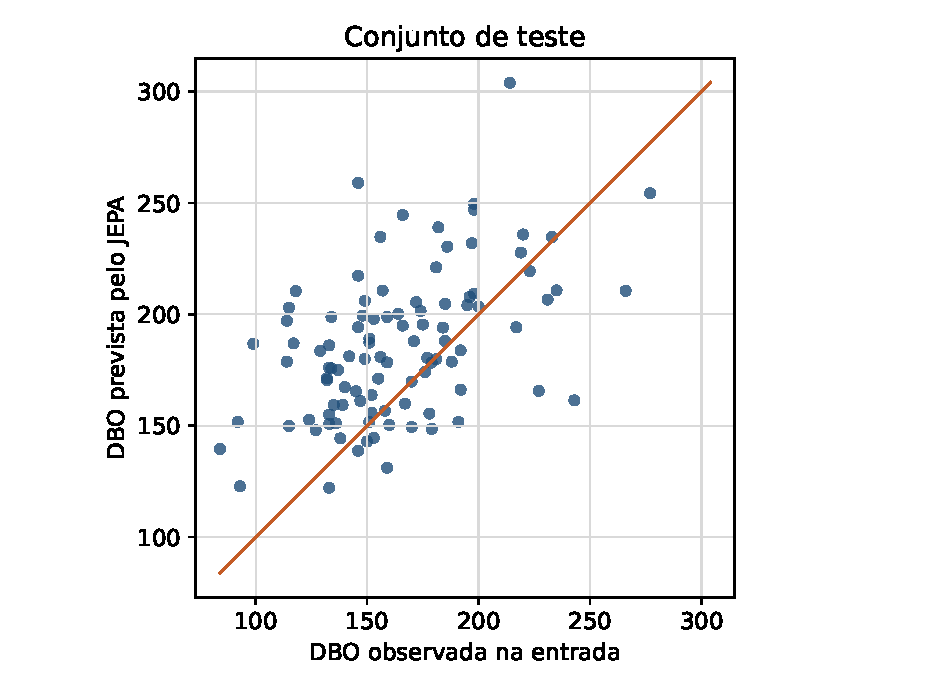
\includegraphics[width=0.72\textwidth]{figuras/jepa_observado_previsto.pdf}
\caption{Teste do JEPA. A nuvem fica acima da reta de igualdade: a previsão segue o nível mais alto do treino.}
\label{fig:previsto}
\end{figure}

\begin{figure}[H]
\centering
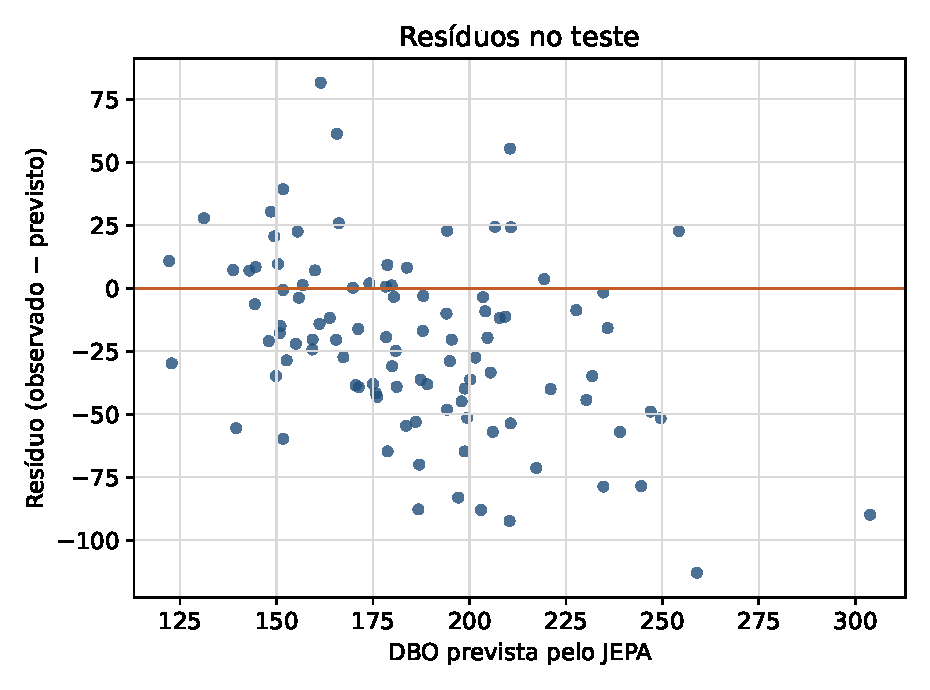
\includegraphics[width=0.72\textwidth]{figuras/jepa_residuos.pdf}
\caption{Resíduos no teste. O centro está abaixo de zero, e o erro cresce nas previsões mais altas.}
\label{fig:residuos}
\end{figure}

\begin{figure}[H]
\centering
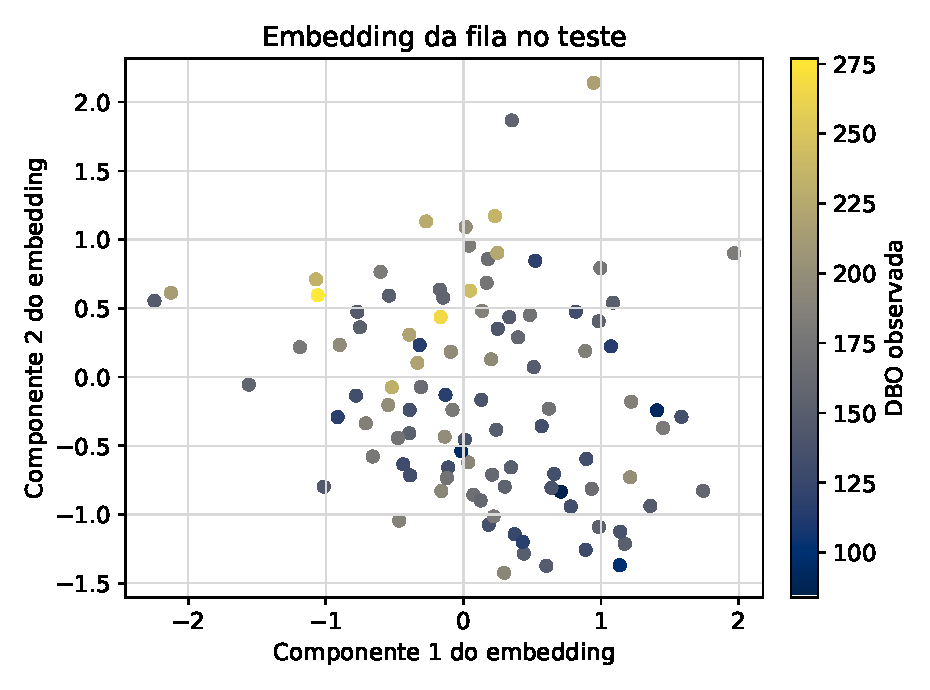
\includegraphics[width=0.78\textwidth]{figuras/jepa_embedding.pdf}
\caption{Embedding da fila no teste, em duas componentes. A cor é a DBO observada. Amarelo e azul dividem as mesmas regiões.}
\label{fig:embedding}
\end{figure}

\section{Leitura}

O JEPA reduz o MAE de 40,88 para 32,78 em relação à média do treino. Fica 0,35 abaixo da reta da leitura atual e 0,78 acima da RNN. O RMSE, 41,39, fica acima dos dois. O \(R^{2}\) de $-$0,28 repete o deslocamento já visto na RNN: o treino vive em torno de 195 e o teste em torno de 164, e a previsão permanece cerca de 22 unidades acima das observações finais.

O treino do embedding não organizou a DBO. A validação escolheu a primeira época porque as épocas seguintes aumentavam o MAE da leitura. O vetor da DBO ficou com desvio 0,061, longe do alvo 1 da penalidade, e a correlação com o vetor previsto é nula. A Figura~\ref{fig:embedding} mostra o mesmo: a cor da DBO não desenha uma escala no plano. A reta de leitura, aplicada a um vetor quase cru, é quem produz o número. Com 1816 parâmetros, o JEPA não separa essa reta nem a RNN de 97 parâmetros.

A Figura~\ref{fig:previsto} e a Figura~\ref{fig:residuos} mostram o mesmo viés do período final. DQO e SST recentes ainda empurram a estimativa para o patamar antigo. Prever o vetor da DBO, em vez do número, não corrige essa mudança de nível.

\section{Conclusão}

Com a fila de 10 leituras, o JEPA chega a MAE 32,78, RMSE 41,39 e \(R^{2}\) $-$0,28 nos 100 dias finais. A RNN, no mesmo corte, chega a MAE 32,00 e RMSE 40,68. A reta da leitura atual chega a MAE 33,13 e RMSE 40,75. O embedding previsto não acompanha o embedding da DBO, e a validação encerra o treino na primeira época. Nesta amostra, a arquitetura preditiva de embeddings não melhora a estimativa.

O notebook é \texttt{modelo/jepa\_dbo\_entrada.ipynb}. A RNN está em \texttt{docs/rnn\_dbo\_entrada.pdf}.
\end{document}
